\documentclass[
12pt,
a4paper,
bibliography=totocnumbered, %Literaturverzereichnis als Eintrag ins Inhaltsverzeichnis
%twoside, %Zweiseitiger Druck
BCOR=1cm, %Platz zum Lochen
oneside, %Einseitiger Druck
]{scrartcl}

\usepackage{geometry}

\usepackage[default]{fontsetup}
%\usepackage[onehalfspacing]{setspace}

\usepackage[ngerman]{babel}
\usepackage[babel=true,german=quotes]{csquotes}

\usepackage{microtype}
\usepackage{mleftright}
%\newcommand{\Le}{\mleft}
%\newcommand{\Ri}{\mright}
\usepackage[no-script, no-scriptscript, no-inner, no-close]{innerscript}

% Mathepakete (unicode-math ersetzt amssymb, amsfonts etc.)
\usepackage{amsmath,amsthm}
\usepackage{mathtools}
\usepackage{fixdif,derivative}
\usepackage{physics2}
\usephysicsmodule{ab.legacy}

\usepackage{unicode-math}
\setmathfont{NewCMMath-Book}
\setmathfont{NewCMMath-Book}[range=cal, StylisticSet=1]
\setmathfont{NewCMMath-Book}[range=scr]

\usepackage{siunitx}
\sisetup{detect-weight=true, detect-family=true,locale=DE,range-phrase={\,bis\,},list-final-separator ={\,\linebreak[0] \text{und}\,},separate-uncertainty=true,per-mode = symbol-or-fraction}
%\SI[per-mode = fraction]{1}{\meter\per\second} erzwingt auch im Fließtext die Bruchdarstellung.
\DeclareSIUnit\curie{Ci}%Zusätzliche Einheit definieren

\usepackage{tabularx, booktabs, multirow}
\usepackage{array}
\usepackage{enumitem}
\usepackage{float}
\usepackage{graphicx}
\usepackage{xurl}

\usepackage[final]{pdfpages}
\usepackage{framed, color} %Framed: Paket, mittels dessen ein Rahmen um einen Bereich definiert werden kann. Color: Lässt Farbdarstellung in Schrift, Hintergrund etc. zu

\usepackage{scrlayer-scrpage} %Header für die KOMA-script-Klasse

%\usepackage[square,numbers]{natbib}
\usepackage{subfigure} %Mehrere Bilder in einer Figure-Umgebung

\usepackage[bookmarks,colorlinks=true]{hyperref}
\hypersetup{
	colorlinks,
	linktocpage,
	citecolor=black,
	filecolor=black,
	linkcolor=black,
	urlcolor=black,
	pdftitle=X,
	pdfauthor=JM-VS
}

\usepackage[backend=biber, style=chem-angew]{biblatex}
\addbibresource{lit.bib}

\numberwithin{equation}{section} % Die Nummerierung von Gleichungen bekommt die jeweilige Section-Nummer als Präfix

\setlength{\parindent}{0pt} %Einrücktiefe von neuen Absätzen
\setlength{\parskip}{6pt} %Abstand von Absätzen

\pagestyle{scrheadings}%Kopf und Fußzeilen
\ohead{\textbf{\GRUPPENNR\ - \VERSUCHSNR}} %Header oben links auf linker Seite (ungerade Seitenzahl) und oben rechts auf rechter Seite (gerade Seitenzahl), beinhaltet gruppennummer und Versuchskürzel. Im Fall eine einseitigen Dokuments: Header oben rechts
\ihead{\VerfasserEINS\;\&\;\VerfasserZWEI} %Header oben rechts auf linker Seite und oben links auf rechter Seite. Beinhaltet die Namen der Verfasser. Im Fall eine einseitigen Dokuments: Header oben links!
\ofoot{\thepage} %Footer unten links auf linker und unten rechts auf rechter Seite, enthält die jeweilige Seitenzahl. Im Fall eines einseitigen Elements: Footer unten rechts!
\cfoot{\empty} %Mittig unten im Footer soll nichts eingetragen werden
\ifoot{\empty} %Footer unten rechts auf linker und unten links auf rechter Seite. Hier ebenfalls leer.

\newcommand{\tz}{T_{\text{II}}}
\newcommand{\ts}{T_{\text{S}}}
\newcommand{\tgl}{T_{\text{gl}}}
\newcommand{\tgeg}{T_{\text{geg}}}
\newcommand{\omz}{\omega_{\text{II}}}
\newcommand{\omgl}{\omega_{\text{gl}}}
\newcommand{\omgeg}{\omega_{\text{geg}}}
\newcommand{\kB}{k_{\text{B}}}
%%%%%%%%%%%%%%%%%%%%%%%%%%%%%%
% GENERAL

\newcommand{\e}{\mathrm{e}} % Der hier von \eul redefined
\newcommand{\imag}{\mathrm{i}}
%\newcommand{\dif}[1]{\mathrm{d}#1} not needed (fixdif package)
\newcommand{\Le}{\mleft}
\newcommand{\Ri}{\mright}
\newcommand{\RR}{\mathbb{R}}
\newcommand{\ensp}{\enspace}
\newcommand{\sbst}{\subset}
\newcommand{\id}{\mathbb{1}}
\renewcommand{\implies}{\Rightarrow}
\newcommand{\openint}[2]{{]{#1,#2}[}}
\newcommand{\diag}[1]{\mathrm{diag}\Le\{#1\Ri\}}
\DeclarePairedDelimiterXPP\Exp[1]{\operatorname{exp}}{(}{)}{}{#1} %exp Operator mit passendem Klammern Spacing oder so
\newcommand{\bv}[1]{\symbfit{#1}} % bolt vector

%%%%%%%%%%%%%%%%%%%%%%%%%%%%%%
% SYMBOLS

\newcommand{\veps}{\varepsilon}
\newcommand{\vphi}{\varphi}

%%%%%%%%%%%%%%%%%%%%%%%%%%%%%%
% TOPOLGY

\DeclareMathOperator{\accumulated}{acc}
\DeclareMathOperator{\isolated}{iso}
\DeclareMathOperator{\interior}{int}
\DeclareMathOperator{\exterior}{ext}
\newcommand{\edge}{\partial}
\DeclareMathOperator{\CauchySeq}{\text{CF}}

%%%%%%%%%%%%%%%%%%%%%%%%%%%%%%
% LINEAR ALGEBRA

\DeclareMathOperator{\trace}{Tr}
\DeclareMathOperator*{\Vektor}{\scalerel*{V}{\sum}}
\DeclareMathOperator{\core}{ker}
%\DeclareMathOperator{\span}{span}

%%%%%%%%%%%%%%%%%%%%%%%%%%%%%%
% VECTOR CALCULUS

\newcommand{\nbl}{\symbfup{\nabla}}
\DeclareMathOperator{\grad}{grad}
\DeclareMathOperator{\divgc}{div}
\DeclareMathOperator{\rot}{rot}

%%%%%%%%%%%%%%%%%%%%%%%%%%%%%%
% PHYSICS
\newcommand{\poiss}[2]{\Le\{#1,#2\Ri\}} % Poissant brackets

%\prime
%\dprime
%\trprime

% Hier können die individuellen Anpassungen vorgenommen werden, die sich auf das Titelblatt und die Kopfzeilen auswirken.

\newcommand{\VERSUCHSDATUM}{01.10.2025}
\newcommand{\PROTOKOLLDATUM}{\today}

\newcommand{\VerfasserEINS}{Julian Molt}
\newcommand{\MatNoEINS}{3803097}
\newcommand{\StudiengangEINS}{Physik}

\newcommand{\VerfasserZWEI}{Valentin Stopper}
\newcommand{\MatNoZWEI}{3774391}
\newcommand{\StudiengangZWEI}{Physik}

\newcommand{\BETREUER}{Simon Krinke}
\newcommand{\GRUPPENNR}{A-016}

\newcommand{\VERSUCHSNR}{M30}
\newcommand{\VERSUCHSNAME}{Erzwungene Schwingung und Resonanz}


\begin{document}

\thispagestyle{empty}

\begin{titlepage}

	\begin{center}
		\Huge{\textbf{\VERSUCHSNR\ -- \VERSUCHSNAME}}\\
		\vspace{10mm}
		\Large{Protokoll zum Versuch des Physikalischen Praktikums I von \\ \textbf{\VerfasserEINS\;\& \VerfasserZWEI}}\\
		\vspace{10mm}
		\Large{Universität Stuttgart}\\
	\end{center}
	\vspace{1cm}
	\begin{center}
		\begin{tabular}{ll}
			\large{Verfasser:}		& \large{\VerfasserEINS\;(\StudiengangEINS),} \\
			& \large{\MatNoEINS} \\
			\vspace{0cm}\\
			& \large{\VerfasserZWEI\;(\StudiengangZWEI),} \\
			& \large{\MatNoZWEI} \\
			\vspace{0cm}\\
			\large{Gruppennummer:}	& \large{\GRUPPENNR} \\
			\vspace{0cm}\\
			\large{Versuchsdatum:}	& \large{\VERSUCHSDATUM} \\
			\vspace{0cm}\\
			\large{Betreuerin:}		& \large{\BETREUER}
		\end{tabular}
	\end{center}
	\vspace{15mm}

	\begin{center}
		Stuttgart, den \PROTOKOLLDATUM
	\end{center}

\end{titlepage}

\thispagestyle{empty}

\tableofcontents

\clearpage %Neue Seite, davor werden alle noch ausstehenden Grafiken/Tabellen platziert.

\renewcommand{\thepage}{\arabic{page}}
\setcounter{page}{1}

% Die erste eckige Klammer ist optional, die darin angegebene Bezeichnung steht im Inhaltsverzeichnis anstelle des hinteren (längeren) Namens.
\section[Versuchsziel]{Versuchsziel und Versuchsmethode}

\section{Grundlagen}

\begin{equation}
	\Psi(t) = \alpha \e^{\imag \omega_0 t} + \beta \e^{- \imag \omega_0 t}
\end{equation}

\section[Messprinzip]{Messprinzip mit Abbild und Versuchsablauf}

%\begin{figure}[H]
%	\centering{\includegraphics[width=0.9\textwidth]{X.jpg}}
%	\caption{X.}
%	\label{fig:X}
%\end{figure}

\section{Messwerte}

%\begin{table}[H]
%	\centering
%	\caption{X. \label{tbl:X}}
%	\begin{tabular}{ll}
%		\toprule
%		X & X \\
%		\midrule
%		X  & X  \\
%		\bottomrule
%	\end{tabular}
%\end{table}

\section{Auswertung}

\section{Zusammenfassung}


%\begin{thebibliography}{999}
%	\bibitem{Quelle} Versuchsanleitung zu \emph{E24 -- Halbleiterdioden} (Abgerufen am 29.09.2025).
%	Online verfügbar unter: \url{https://www3.physik.uni-stuttgart.de/studium/praktika/ap/pdf_dateien/E24.pdf}
%\end{thebibliography}

\printbibliography

\section{Anhang}

%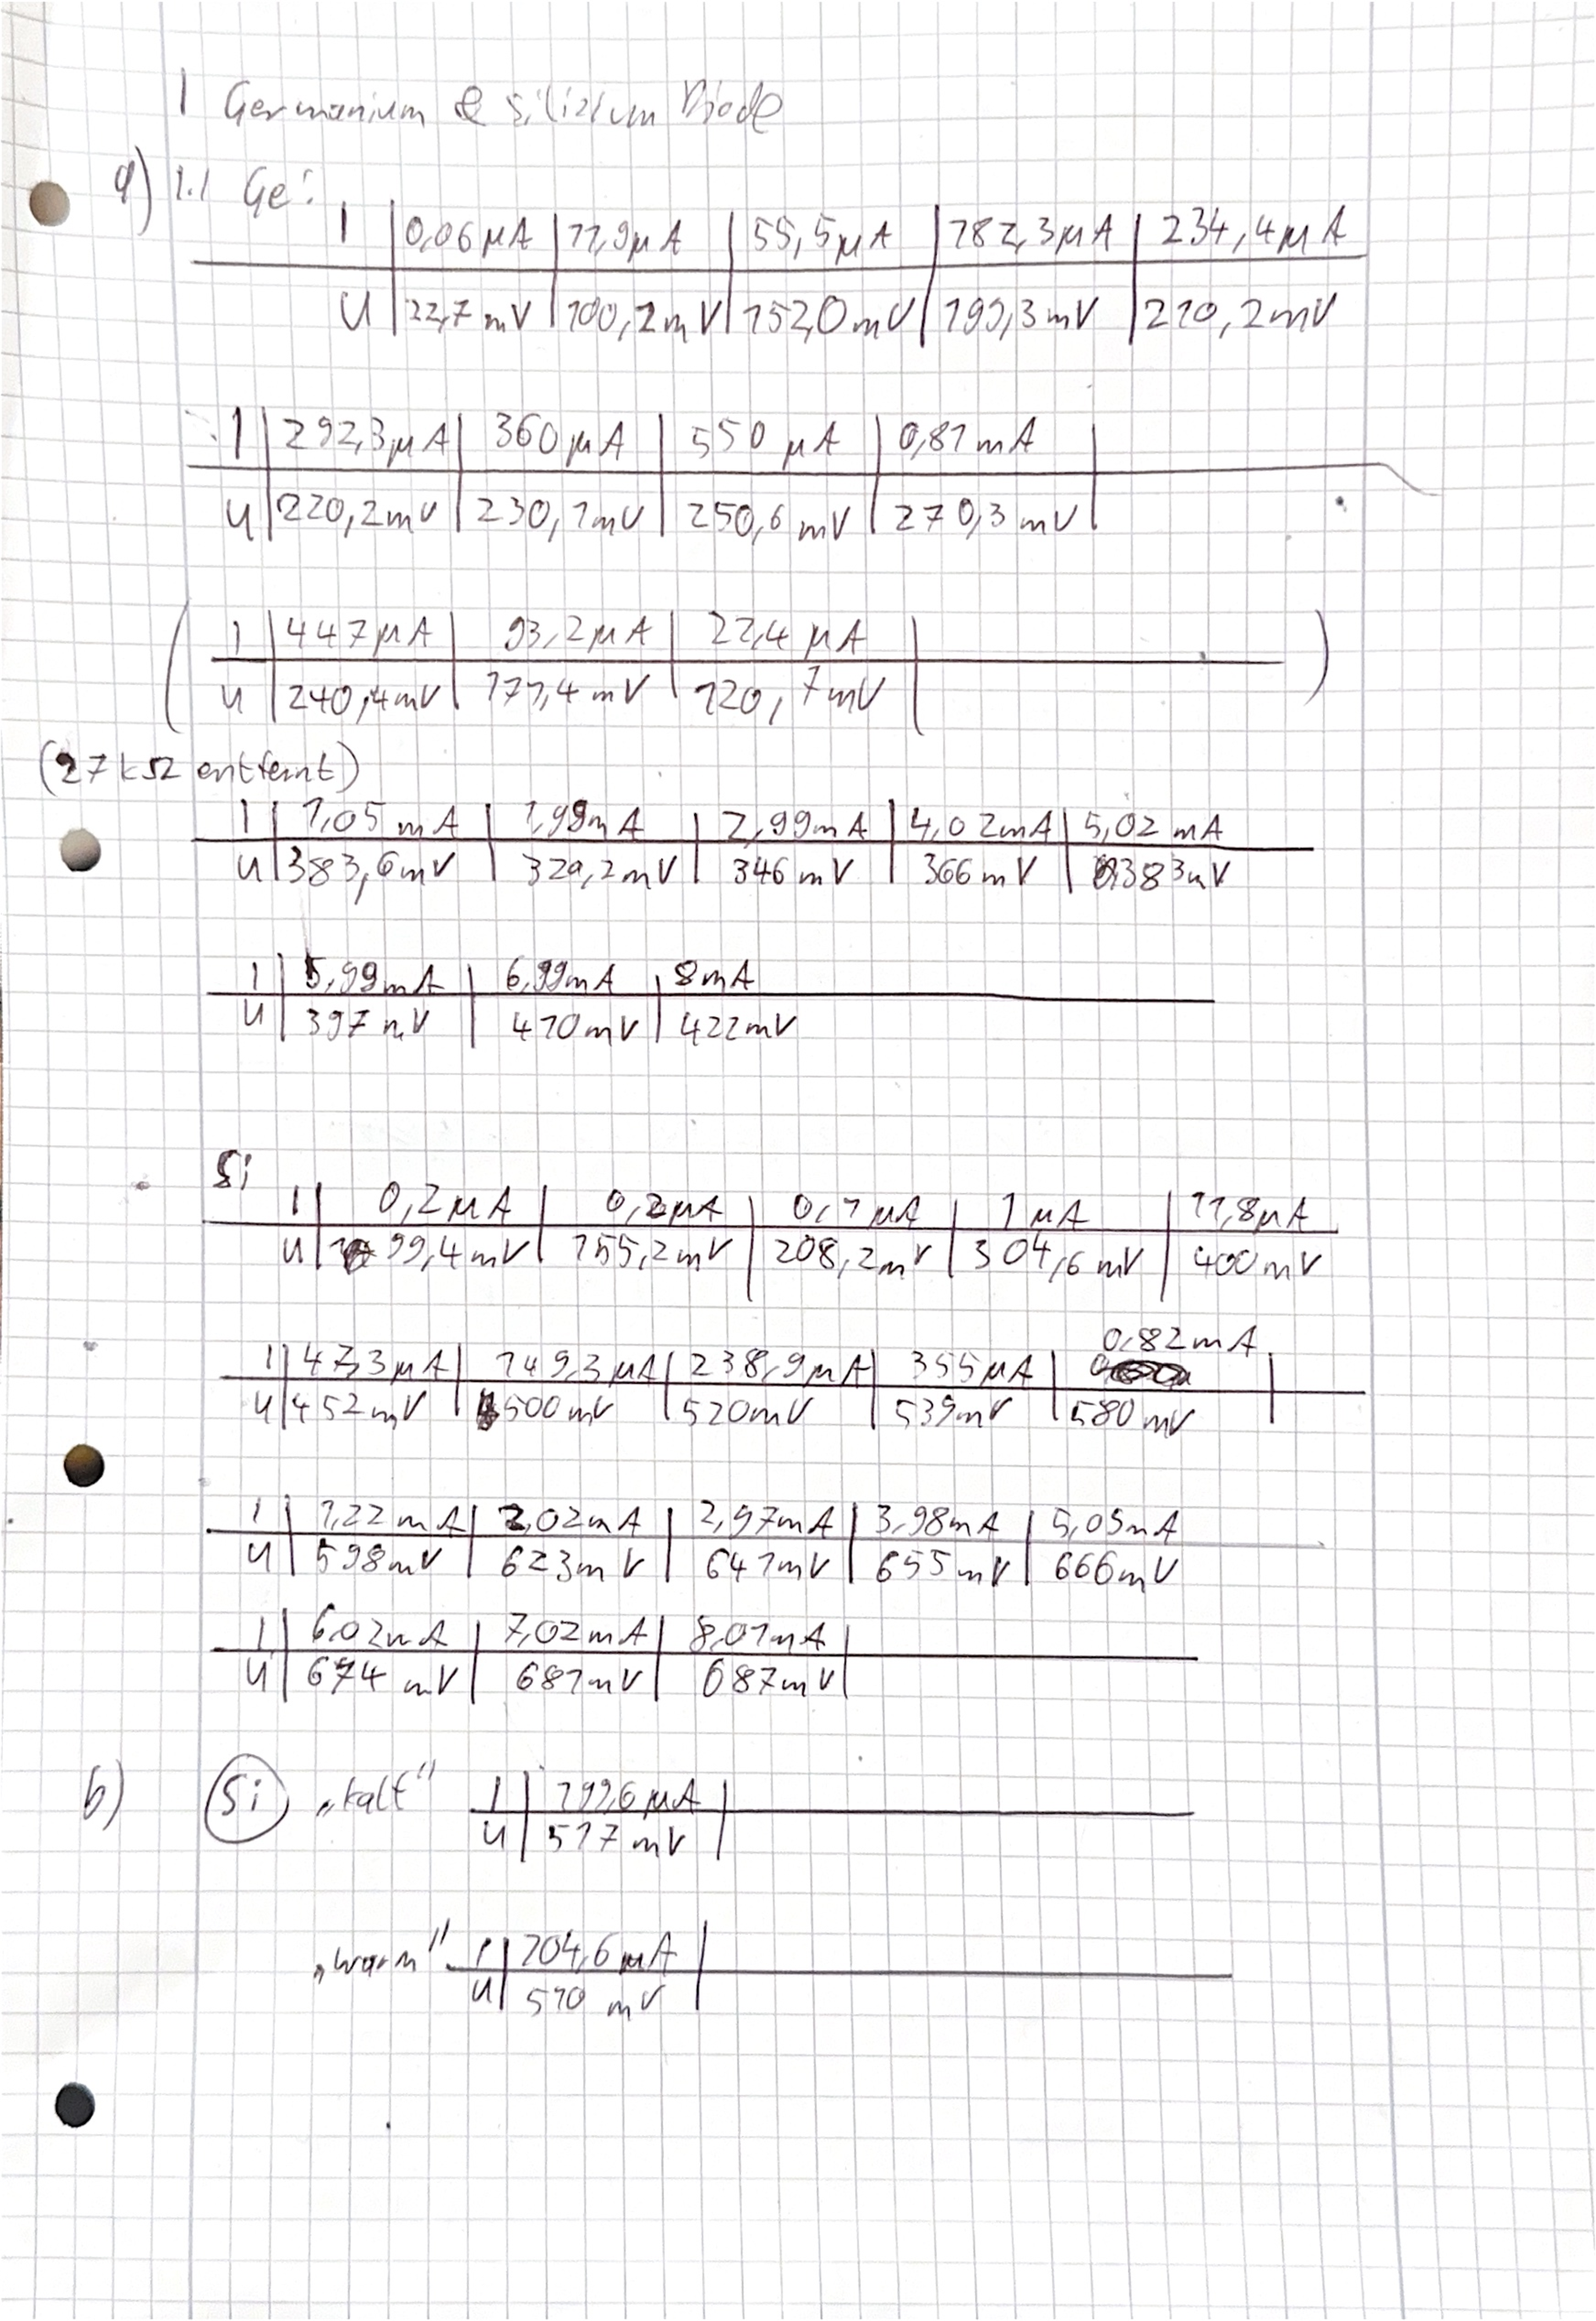
\includepdf[pages=-]{MessprotDioden.pdf}

\end{document}